\documentclass[border={0.1cm 0.1cm 0.1cm 0.1cm}]{standalone}  %E,S,W,N

\usepackage{amssymb}
\usepackage{amsmath}
\usepackage{tikz}

\begin{document}
	
	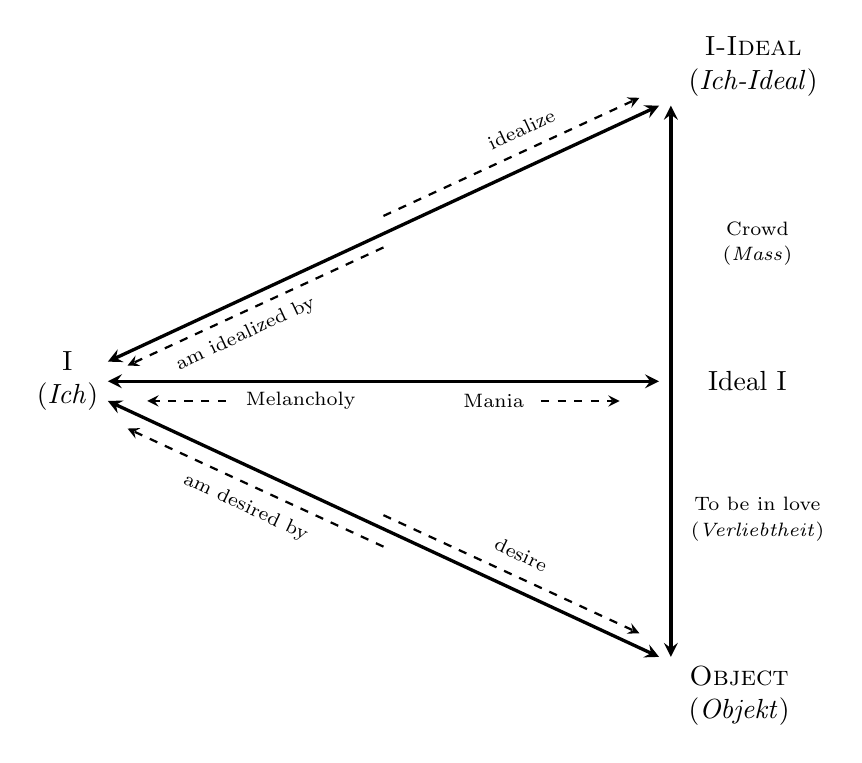
\begin{tikzpicture}	
	\def\s{7} %width of triangle
	
	\node[align=center,left] at (0,0) {I \\ (\textit{Ich})};
	\node[align=left,right] at (\s+0.5,0) {Ideal I};
	\node[align=center] at (\s+1.25,0.25*\s) {\scriptsize Crowd\\[-1mm] \scriptsize (\textit{Mass})};
	\node[align=center] at (\s+1.25,-0.25*\s) {\scriptsize To be in love\\[-1mm] \scriptsize (\textit{Verliebtheit})};
	\node[align=center,above right] at (\s+0.25,0.5*\s) {\textsc{I-Ideal} \\ (\textit{Ich-Ideal})};
	\node[align=center,below right] at (\s+0.25,-0.5*\s) {\textsc{Object} \\ (\textit{Objekt})};
	
	%MAIN ARROWS
	\draw[very thick,<->,>=stealth] (0,0.25)--(\s,0.5*\s);
	\draw[very thick,<->,>=stealth] (0,0)--(\s,0);
	\draw[very thick,<->,>=stealth] (0,-0.25)--(\s,-0.5*\s);
	\draw[very thick,<->,>=stealth] (\s+0.15,0.5*\s)--(\s+0.15,-0.5*\s);
	
	%DASHED ARROWS
	\draw[thick,->,>=stealth,dashed] (0.5*\s,1.35+0.75)--++(0.5*\s-0.25,1.5);
	\node at (0.75*\s,3.2) {\rotatebox{25}{\scriptsize idealize}};
	\draw[thick,->,>=stealth,dashed] (0.5*\s,1.25+0.45)--++(-0.5*\s+0.25,-1.5);
	\node at (0.25*\s,0.6) {\rotatebox{25}{\scriptsize am idealized by}};
	%
	\draw[thick,->,>=stealth,dashed] (0.5*\s,-1.25-0.45)--++(0.5*\s-0.25,-1.5);
	\node at (0.75*\s,-2.2) {\rotatebox{-25}{\scriptsize desire}};
	\draw[thick,->,>=stealth,dashed] (0.5*\s,-1.35-0.75)--++(-0.5*\s+0.25,1.5);
	\node at (0.25*\s,-1.6) {\rotatebox{-25}{\scriptsize am desired by}};
	
	\node at (0.35*\s,-0.25) {\scriptsize Melancholy};
	\draw[thick,->,>=stealth,dashed] (1.5,-0.25)--++(-1,0);
	\node at (0.7*\s,-0.25) {\scriptsize Mania};
	\draw[thick,->,>=stealth,dashed] (5.5,-0.25)--++(1,0);
	
	%\draw[help lines] (-1,-3) grid (6,3);
	\end{tikzpicture}
	
\end{document}